\documentclass[12pt]{article}
\usepackage[a4paper, total={6.5in, 8in}]{geometry}
\usepackage{xargs}
\usepackage{amsmath,amssymb}
\usepackage{hyperref}
\usepackage{physics}
\usepackage{graphicx}

\begin{document}

	\title{Development and application of new coherent state based methods of quantum dynamics\\\hfill\\First Formal Progress Report}
	\author{Michal Horanský}
	\maketitle
	
	\tableofcontents
	
	\section{Introduction}
	The following document is an FFPR for the post-graduate research project on coherent states the author does under the supervision of Professor Dmitry Shalashilin and Professor Orde Munro. The project aims to contribute theoretical framework for fast simulation of quantum dynamics for the COSMOS research group.
	\subsection{Coherent states}
	The task of solving the time-dependent Schrodinger equation numerically on a system with a large number of degrees of freedom $M$ runs into the problem of time complexity, which scales exponentially with $M$ \cite[Sec. 1.2]{curse_of_dimensionality}. A possible circumvention of this problem lies in utilising a semi-classical approach, where a basis of states evolving "classically" according to the Hamiltonian is chosen, and decomposing the wavefunction into this basis allows one to study the extent of quantum coupling. Schrodinger used this idea in 1926 to formulate the "classical states" of the harmonic oscillators \cite{harmonic_classical_states}, and remarked on their useful properties: the expected values of $\hat{x}$ and $\hat{p}$ follow 	the classical equations of motion, and the uncertainty $\Delta x\Delta p$ does not increase in time.
	
	Glauber, in 1963, applied the same idea to the Hamiltonian which describes the interaction between an atomic system and an electromagnetic field, forming field coherent states\footnote{Also known as Glauber coherent states.}, and showed that, although not orthogonal, they form a complete basis of the Hilbert space, they minimise uncertainty, and remain coherent under time evolution \cite{field_coherent_states}. Glauber constructed three equivalent definitions of field coherent states $\ket{\alpha}$ of a single mode:
	\begin{itemize}
		\item Eigenstates of the annihilation operator
		$$\hat{a}\ket{\alpha} = \alpha\ket{\alpha}$$
		\item Minimum-uncertainty states.
		\item Displacements of the ground state
		$$\ket{\alpha} = \exp(\alpha\hat{a}^\dagger-\alpha^*\hat{a})\ket{0}$$
	\end{itemize}
	
	Attempting to generalise Glauber's construction to an arbitrary Hamiltonian restricts our approach. Firstly, constructing coherent states as eigenstates of the lowering operator is trivially impossible on finite-dimensional Hilbert spaces. Secondly, constructing coherent states as minimum-uncertainty states is ill-advised, as it is not necessary they form a complete basis, or that unity can be resolved in them \cite{no_unity}. Constructing coherent states as a displacement of some reference state, however, is always possible, and a satisfactory group-theoretical formulation was found independently by Perelomov \cite{perelomov_og} and Gilmore \cite{gilmore_og} in 1972. This construction follows these steps:
	\begin{enumerate}
		\item Find the action group $G$ of the system, i.e. a Lie group such that both the Hamiltonian and the transition operators can be expressed as functions of the elements of the Lie algebra of $G$.
		\item Choose a reference state $\ket{\Phi_0}$ in the Hilbert space (typically the ground state or some other extremal state).
		\item Find the stability subgroup $H\subset G$ which is the group of all elements of $G$ which leave the reference state invariant up to a phase factor.
		\item Find the quotient group $G/H$. Each element $\Omega\in G/H$ generates a unique coherent state $\Omega\ket{\Phi_0}$, and the resulting set of coherent states is topologically equivalent to the coset space $G/H$.
	\end{enumerate}
	This process, as presented and discussed by Zhang, Feng, and Gilmore \cite{ZFG}, constructs a basis of states which retain all the desired properties (coherence, minimal uncertainty, and evolution according to an effective classical Hamiltonian), and which can be constructed for a system with any dynamical group. Unity can always be resolved in this basis, which is complete but not orthogonal, and therefore overcomplete.
	
	Moreover, if the Lie algebra of the dynamical group is semisimple, it can be transformed into the Cartan basis, where all operators in the algebra are either fully diagonal, or analogous to the creation and annihilation operators. Viscondi, Grigolo, and de Aguiar found an expression for the semiclassical propagator for such cases, which determines the overlap of two different coherent states at different times \cite{Aguiar}. Here the full picture of the semiclassical approximation is painted: the coherent states evolve according to equations of motion governed by an effective classical Hamiltonian, and the amplitude of their overlap measures their entanglement.
	
	\subsection{Bosonic quantum dynamics}\label{sec:two applications}
	The semiclassical approach is firstly applied to bosonic systems with constant total particle number. As shown in Sec. \ref{sec:sum}, all such systems possess the same dynamical group, and thus one construction of coherent states can be used to all such systems.
	
	The approach is applied to two particular systems:
	\begin{enumerate}
		\item The multimode Bose-Hubbard model, which is useful in description of optical lattices \cite{optical_lattices}.
		\item A displaced harmonic trap, which is used as a benchmark for the efficiency of the approach for a large number of modes.
	\end{enumerate}
	The two systems have been previously studied by 1. Qiao and Grossmann \cite{grossmann} and 2. Green and Shalashilin \cite{green}, respectively.
	
	Qiao and Grossmann apply a similar approach to mine in their study of the Bose-Hubbard model, constructing coherent states from the $SU(M)$ dynamical group. However, they use normalised coherent states, for which the derivation of the equations of motion is slightly different, and they do not posses some desirable properties, such as a complex quotient-space metric, due to the fact they are not analytic.
	
	Green and Shalashilin do not use the group-theoretical $SU(M)$ coherent states. Rather, they use "coupled coherent states", which, as eigenstates of the annihilation operator, are analogous to field coherent states. These coupled coherent states are not eigenstates of the total particle number, and as such are not contained in the Hilbert space of the system, which renders them inefficient as a basis.
	
	The aim of the first part of my project is to reproduce the results of these two investigations using analytic unnormalised $SU(M)$ coherent states based on the construction demonstrated by Viscondi, Grigolo, and de Aguiar. This would prove the efficiency and accuracy of the new group-theoretical approach to semiclassical methods, and pave the way for further work on other systems, namely fermionic quantum dynamics.
	
	\section{Theory: SU(M) coherent states} \label{sec:sum}
	
	Any second-order\footnote{Comprising of one-body and two-body interactions} Hamiltonian for a bosonic system with $M$ modes which preserves the total particle number can be formulated in second-quantisation in the following general form \cite[p. 3]{green}:
	\begin{equation}\label{eq:general hamiltonian}
	\hat{H} = \sum_{\alpha=1}^M\sum_{\beta=1}^M V^{(1)}_{\alpha\beta}\hat{a}^\dagger_\alpha\hat{a}_\beta + \frac{1}{2}\sum_{\alpha=1}^M\sum_{\beta=1}^M\sum_{\gamma=1}^M\sum_{\delta=1}^M V^{(2)}_{\alpha\beta\gamma\delta}\hat{a}^\dagger_\alpha\hat{a}^\dagger_\beta\hat{a}_\gamma\hat{a}_\delta
	\end{equation}
	where $V^{(1)}_{\alpha\beta}, V^{(2)}_{\alpha\beta\gamma\delta}$ are the matrix elements of the one-body and two-body interaction, respectively.
	
	For a total number of particles $S$, the Hilbert space is spanned by occupancy eigenstates
	\begin{equation}\label{eq:occ_basis}
	\ket{s_1,s_2\dots s_M}\qq{where} s_1+s_2+\dots + s_M = S
	\end{equation}
	
	\subsection{Quotient group $G/H$ for bosonic systems preserving total particle number}
	
	We see that the transition operators for the occupancy basis in Eq. \ref{eq:occ_basis} are
	\begin{equation}
		\hat{T}_{ij}=\hat{a}^\dagger_i\hat{a}_j
	\end{equation}
	and the Hamiltonian can be expressed as a second-order polynomial in terms of $\hat{T}_ij$. Finally, we see that
	\begin{equation}
	\left[\hat{T}_{ij}, \hat{T}_{i'j'}\right]=\hat{T}_{ij'}\delta_{i'j}-\hat{T}_{i'j}\delta_{ij'}
	\end{equation}
	therefore $\hat{T}_{ij}$ forms a Lie algebra. We transform this basis like so:
	\begin{eqnarray*}
	\hat{S}&=&\sum_{i=1}^M\hat{T}_{ii}\\
	\hat{H}_i&=&\hat{T}_{i+1,i+1}-\hat{T}_{ii}\qq{for}i=1,2\dots M-1\\
	\hat{E}_{ij}&=&\hat{T}_{ij}\qq{for}i>j\\
	\hat{E}_{ij}^\dagger &=&\hat{T}_{ji}\qq{for}i>j
	\end{eqnarray*}
	We see that the element $\hat{S}$ commutes with every other element, and therefore the dynamical group can be expressed as the direct product of $U(1)$ and the group generated by $\hat{H},\hat{E},\hat{E}^\dagger$. This second group's Lie algebra constitutes the complete matrix basis for real traceless $(M\times M)$ matrices, and therefore the second group is $SL(M,\mathbb{R})$. The full dynamical group is therefore $U(1)\otimes SL(M,\mathbb{R})$
	
	We now choose a reference state. We will choose
	\begin{equation}
	\ket{\Phi_0}=\ket{0,0\dots S}
	\end{equation}
	This state is conventional in literature on $SU(M)$ coherent states, and is suitable for a specific reason: it is extremal in the sense that operators $S, H$ leave it invariant up to a phase factor and operators $\hat{E}$ destroy it. Therefore we identify the general element of the quotient group $G/H$ as
	\begin{equation} \label{eq:quotient element}
	\hat{\Omega}(\vec{z})=\sum_i^{M-1}z_i\hat{E}^\dagger_{M,i}=\sum_i^{M-1}z_i\hat{a}^\dagger_i\hat{a}_M
	\end{equation}
	where $\vec{z}$ is an $(M-1)$-dimensional complex vector.
	
	\subsubsection{On the difference between $SU(M)$ and $SL(M,\mathbb{R})$}
	When transforming the basis $\hat{T}_{ij}$, one may choose to complexify it and form a set of Hermitian and anti-Hermitian operators ($\hat{T}_{ij}+\hat{T}_{ji}$ and $i(\hat{T}_{ij}-\hat{T}_{ji})$), respectively. This complexification is allowed in the sense that the transition operators remain independent even if the field of coefficients is complex. Identifying the resulting operators with the generalised Gell-Mann matrices yields the dynamical group $SU(M)$ \cite{gellmann}. Although resulting in a different quotient group $G/H$, the coherent states are identical to our $SL(M,\mathbb{R})$ construction. For the details of this construction, see Sec. 2.2.3 in the paper by Viscondi, Grigolo, and de Aguiar \cite{Aguiar}.
	
	Also note that the extra factor $U(1)$ in the dynamical group is commonly ignored in literature, since it is trivially included in the stability subgroup, and therefore does not affect the construction of the coherent states.
	
	
	\subsection{Construction and properties}
	Applying the quotient elements from Eq. \ref{eq:quotient element} to the reference state we obtain the coherent states
	\begin{equation}\label{eq:exponential form}
	\ket{\vec{z}}=\exp(\sum_i^{M-1}z_i\hat{a}^\dagger_i\hat{a}_M)\ket{\Phi_0}
	\end{equation}
	This expression can be simplified \cite{buonsante} into the following form:
	\begin{equation}
	\ket{\vec{z}}=\frac{1}{\sqrt{S!}}\left(\hat{a}^\dagger_M+\sum_i^{M-1}z_i\hat{a}^\dagger_i\right)^S\ket{0,0\dots 0}
	\end{equation}
	
	Note that these states are, in general, not normalised. Therefore, I will denote unnormalized coherent states with curly brackets in the bra-ket notation, following the convention in \cite{Aguiar}, like so:
	\begin{equation} \label{eq:canonical form}
	\unnormket{\vec{z}}=\frac{1}{\sqrt{S!}}\left(\hat{a}^\dagger_M+\sum_i^{M-1}z_i\hat{a}^\dagger_i\right)^S\ket{0,0\dots 0}
	\end{equation}
	The approach of Qiao and Grossmann uses a slightly different form, which imposes an extra condition to have the basis states normalised. However, this extra condition has to be accounted for in the equations of motion, which they do not do, as they expect the states to remain normalised under time evolution. This leads to overparametrisation, which is not only inefficient, but renders the construction of a quotient-space metric or identity operator in their formalism ill-formed. Viscondi, Grigolo, and de Aguiar take the unnormalized states $\unnormket{z}$ and project them onto a normalised space of equal dimension by adding a normalisation coefficient. However, since this coefficient depends on both $\vec{z}$ and $\vec{z}^*$, the normalised states are not analytic. I take a different approach: I work directly with the unnormalised states as basis vectors, and include a normalisation factor in the Lagrangian, which still permits me to use Wirtinger calculus to find the equations of motion.
	\subsubsection{Relationship between the coherent state and occupancy bases}
	By applying the multinomial theorem to Eq. \ref{eq:canonical form} we obtain the decomposition of $\unnormket{z}$ into the occupancy basis:
	\begin{equation}
	\unnormket{z}=\sum_{k_1+k_1+\dots +k_M=S}\sqrt{\frac{S!}{k_1!k_2!\dots k_M!}}z_1^{k_1}z_2^{k_2}\dots z_{M-1}^{k_{M-1}}\ket{k_1,k_2\dots k_M}
	\end{equation}
	
	\subsubsection{Overlaps and reduced forms}
	By applying Wick's theorem to Eq. \ref{eq:canonical form} we obtain the overlap element:
	\begin{equation}\label{eq:overlap}
	\unnormbraket{\vec{z}_a}{\vec{z}_b}=\left(1+\vec{z}_a^*\cdot\vec{z}_b\right)^S
	\end{equation}
	Since unmatched creation and annihilation operators are not members of the dynamical Lie algebra, acting with them on the coherent states projects them outside of the Hilbert space. We can describe this with the reduced form of $\unnormket{\vec{z}}$, defined as follows:
	\begin{eqnarray}
	\unnormket{\vec{z}'}&=&\unnormket{z}\qq{where}S'=S-1\\
	\unnormket{\vec{z}^{(r)}}&=&\unnormket{z}\qq{where}S'=S-r
	\end{eqnarray}
	and we have
	\begin{equation}
	\hat{a}_i\unnormket{\vec{z}}=\sqrt{S}z_i\unnormket{\vec{z}'}
	\end{equation}
	Therefore, the matrix element of a normal-ordered product of a set of transition operators is evaluated as follows:
	\begin{equation}\label{eq:reduced overlap}
	\unnormmel{\vec{z}_a}{\hat{a}^\dagger_{i_1}\dots \hat{a}^\dagger_{i_r}\hat{a}_{j_1}\dots \hat{a}_{j_r}}{\vec{z}_b}=\begin{cases}
	\frac{S!}{(S-r)!}\prod_{k=1}^r z^*_{a,i_k}z_{b,j_k}\unnormbraket{\vec{z}_a^{(r)}}{\vec{z}_b^{(r)}} & r \leq S\\
	0 & r > S
	\end{cases}
	\end{equation}
	In the above cases, we take as convention $z_M=1$, which extends the vector without adding an extra degree of freedom, and allows for a more concise form for many equations. From this point onwards, assume this is the case in every equation unless otherwise stated.
	
	For convenience, we will also define the reduced overlap matrix
	\begin{equation}
	X^{(r)}_{ab}=\unnormbraket{\vec{z}^{(r)}_a}{\vec{z}^{(r)}_b}=\left(1+\vec{z}_a^*\cdot\vec{z}_b\right)^{S-r}
	\end{equation}
	
	\subsubsection{Derivatives}
	Using the form in Eq. \ref{eq:exponential form}, we immediately see
	\begin{eqnarray}
	\pdv{z_i}\unnormket{\vec{z}}&=&\hat{a}^\dagger_i\hat{a}_M\unnormket{\vec{z}}\\
	\pdv{z^*_i}\unnormket{\vec{z}}&=&0
	\end{eqnarray}
	The time derivative can be expanded into these partial derivatives, yielding
	\begin{equation}\label{eq:time derivative}
	\dv{t}\unnormket{\vec{z}}=\left(\sum_{i=1}^{M-1}\dot{z}_i\hat{a}^\dagger_i\hat{a}_M\right)\unnormket{\vec{z}}
	\end{equation}
	
	\subsubsection{Identity}
	Following the approach in \cite{Aguiar}, the identity operator on the quotient space is
	\begin{equation}\label{eq:continuous identity}
	\hat{I}=\int \frac{(S+M-1)!}{S!\left(1+\vec{z}^*\cdot\vec{z}\right)^{S+M}}\unnormket{\vec{z}}\unnormbra{\vec{z}}\frac{\dd^2\vec{z}}{\pi^{M-1}}
	\end{equation}
	
	However, since we work with a discrete sample of the coherent states as a basis, in actuality we will use the inverse overlap matrix as an identity operator, which will allow us to decompose the initial state of the wavefunction into the basis coherent states.
	
	\subsection{Decomposition of the Schrodinger equation}
	Consider a (normalized) wavefunction decomposed into a basis of coherent states:
	\begin{equation}\label{eq:decomposition}
	\ket{\Psi(t)}=\sum_{a\in\text{basis}}A_a\unnormket{\vec{z}_a}
	\end{equation}
	The Lagrangian form of the Schrodinger equation is as follows\cite{grossmann}:
	\begin{equation}\label{eq:general lagrangian}
	L(t)=\frac{\frac{i}{2}\left(\braket*{\Psi}{\dot{\Psi}}-\braket*{\dot{\Psi}}{\Psi}\right)-\mel{\Psi}{\hat{H}}{\Psi}}{\braket{\Psi}{\Psi}}
	\end{equation}
	However, the wavefunction is initially normalised, and, evolving according to the Schrodinger equation, it therefore remains normalised, and therefore we can omit the normalisation factor, even though we will express this Lagrangian in terms of unnormalised basis vectors.
	
	\subsubsection{Fully variational method}\label{sec:variational}
	In the fully variational method, the time evolution of all general coordinates is coupled together.
	
	We want to express the Lagrangian in Eq. \ref{eq:general lagrangian} as a function of our general coordinates, which are the decomposition coefficients $A_a(t)$ and the coherent state complex elements $z_{a,i}(t)$. Applying Eq. \ref{eq:decomposition} to Eq. \ref{eq:general lagrangian} and expanding yields
	\begin{align}\label{eq:full lagrangian}
	\begin{split}
	L=\frac{i}{2}\sum_{a,b\in\text{basis}}(A_a^*\dot{A}_b-\dot{A}_a^*A_b)\unnormbraket{\vec{z}_a}{\vec{z}_b}+\frac{i}{2}S\sum_{a,b\in\text{basis}}A_a^*A_b\sum_{i=1}^{M-1}(z_{a,i}^*\dot{z}_{b,i}-\dot{z}^*_{a,i}z_{b,i})\unnormbraket{\vec{z}_a'}{\vec{z}_b'}\\
	-\sum_{a,b\in\text{basis}}A_a^*A_b\unnormmel{\vec{z}_a}{\hat{H}}{\vec{z}_b}
	\end{split}
	\end{align}
	Applying the Euler-Lagrange equation to Eq. \ref{eq:full lagrangian} yields the equations of motion:
	\begin{align}
	i\sum_{b\in\text{basis}}\dot{A}_b\unnormbraket{\vec{z}_a}{\vec{z}_b}+iS\sum_{b\in\text{basis}}A_b\sum_{i=1}^{M-1}z_{a,i}^*\dot{z}_{b,i}\unnormbraket{\vec{z}_a'}{\vec{z}_b'}=\sum_{b\in\text{basis}}A_b\unnormmel{\vec{z}_a}{\hat{H}}{\vec{z}_b}\qq{for}&a\in\text{basis}\\
	\begin{split}
	iSA_a^*\sum_{b\in\text{basis}}\left(\dot{A}_b z_{b,i}\unnormbraket{\vec{z}'_a}{\vec{z}'_b}+A_b\dot{z}_{a,i}\unnormbraket{\vec{z}'_a}{\vec{z}'_b}+(S-1)A_b\sum_{j=1}^{M-1}z_{a,j}^*\dot{z}_{b,j}z_{b,i}\unnormbraket{\vec{z}''_a}{\vec{z}''_b}\right)&\\
	=A_a^*\sum_{b\in\text{basis}}A_b\pdv{z^*_{a,i}}\unnormmel{\vec{z}_a}{\hat{H}}{\vec{z}_b}\qq{for}a\in\text{basis,  } i=1,2\dots &M-1
	\end{split}
	\end{align}
	For a basis of size $N$, there are $M\cdot N$ linear equations of motion, which can be expressed in a vectorial form for the following coordinate vector:
	\begin{equation}
	\vec{Q}=\mqty(\vec{Q}_A\\\vec{Q}_z),\qq{where}\vec{Q}_A=\mqty(A_1\\\vdots\\A_N)\qq{and}\vec{Q}_z=\mqty(z_{1,1}\\z_{2,1}\\\vdots\\z_{N,1}\\z_{1,2}\\\vdots\\z_{N,M-1})
	\end{equation}
	The equations of motion are then expressable as
	\begin{equation}\label{eq:variational eqns of motion}
	\begin{split}
	\mqty(X & Y\\Y^\dagger & Z)&\mqty(\dv{t}\vec{Q}_A\\\dv{t}\vec{Q}_z)=-i\mqty(\vec{R}_A\\\vec{R}_z)\\
	\qq{where}&Y_{a,Ni+b}=Sz^*_{a,i}A_b X'_{ab}\\
	&Z_{Ni+a,Nj+b}=A^*_a A_b \left(S(S-1)X_{ab}''z_{a,j}^* z_{b,i}+\delta_{ij}SX_{ab}'\right)\\
	&(R_A)_a=\sum_{b\in\text{basis}}A_b\unnormmel{\vec{z}_a}{\hat{H}}{\vec{z}_b}\\
	&(R_z)_{Ni+a}=A_a^*\sum_{b\in\text{basis}}A_b\pdv{z_{a,i}^*}\unnormmel{\vec{z}_a}{\hat{H}}{\vec{z}_b}
	\end{split}
	\end{equation}
	Finally, we use Eq. \ref{eq:general hamiltonian} to express $\vec{R}_A,\vec{R}_z$ using $V^{(1)},V^{(2)}$:
	\begin{align}
	\unnormmel{\vec{z}_a}{\hat{H}}{\vec{z}_b}&=SX_{ab}'\sum_{\alpha=1}^M\sum_{\beta=1}^MV^{(1)}_{\alpha\beta}z^*_{a,\alpha}z_{b,\beta}+\frac{1}{2}S(S-1)X_{ab}''\sum_{\alpha=1}^M\sum_{\beta=1}^M\sum_{\gamma=1}^M\sum_{\delta=1}^M V^{(2)}_{\alpha\beta\gamma\delta}z^*_{a,\alpha}z^*_{a,\beta}z_{b,\gamma}z_{b,\delta}\notag\\
	\begin{split}
	\pdv{z_{a,i}^*}\unnormmel{\vec{z}_a}{\hat{H}}{\vec{z}_b}&=S(S-1)X_{ab}''z_{b,i}\sum_{\alpha=1}^M\sum_{\beta=1}^M V^{(1)}_{\alpha\beta}z^*_{a,\alpha}z_{b,\beta}+SX_{ab}'\sum_{\beta=1}^M V^{(1)}_{i\beta}z_{b,\beta}\\
	&+\frac{1}{2}S(S-1)(S-2)X_{ab}'''z_{b,i}\sum_{\alpha=1}^M\sum_{\beta=1}^M\sum_{\gamma=1}^M\sum_{\delta=1}^M V^{(2)}_{\alpha\beta\gamma\delta}z^*_{a,\alpha}z^*_{a,\beta}z_{b,\gamma}z_{b,\delta}\\
	&+\frac{1}{2}S(S-1)X_{ab}''\sum_{\beta=1}^M\sum_{\gamma=1}^M\sum_{\delta=1}^M \left(V^{(2)}_{i\beta\gamma\delta}+V^{(2)}_{\beta i\gamma\delta}\right)z^*_{a,\beta}z_{b,\gamma}z_{b,\delta}
	\end{split}
	\end{align}
	
	\subsubsection{Decoupled basis propagation}\label{sec:decoupled equations of motion}
	The fully variational method is "efficient" in the sense that the coupling between the basis vectors is informed by the decomposition coefficients. However, the number of simultaneous equations is $M\cdot N$, so in each step of iteration we need to invert a square matrix with $M\cdot N$ rows, rendering the process slow. An alternative to this is to utilise one of the main properties of coherent states: they evolve along classical trajectories. The advantage is that we need to first solve $N$ systems of $M-1$ equations, and then one system with $N$ equations for the decomposition coefficient propagation. The disadvantage is that a basis sampled suitably for the initial conditions may not be suitable at all points in time, since the decoupled basis may "dissipate" in the quotient space, becoming too sparse. Therefore, intelligent sampling is essential for this approach.
	
	In the decoupled basis propagation approach, we first propagate each element $\unnormket{\vec{z}}$ of our basis set. To find the equations of motion, we cannot omit the normalisation factor in the Lagrangian. There are two ways to go around is:
	\begin{enumerate}
		\item We can add a single normalisation coefficient $A(t)$ to the general coordinates, so that $\ket{\Psi}=A\unnormket{\vec{z}}$. To find the equations of motion for this coordinate system, we can use Eq. \ref{eq:variational eqns of motion} with $N=1$.
		\item We can use the result from \cite{Aguiar} for the classical trajectory of the normalised state
		\begin{equation}
		\dot{\vec{z}}=-i(g^{-1})^T\pdv{\vec{z}}\frac{\unnormmel{\vec{z}}{\hat{H}}{\vec{z}}}{\unnormbraket{\vec{z}}{\vec{z}}}\qq{where}g_{ij}=S\frac{(1+\vec{z}^*\cdot \vec{z})\delta_{ij}-z^*_iz_j}{(1+\vec{z}^*\cdot \vec{z})^2}
		\end{equation}
		Here, $g_{ij}$ is the metric of the quotient space, as derived in Sec. 2.2.3 in \cite{Aguiar}.
	\end{enumerate}
	
	After propagating every element of the basis set, we propagate the decomposition coefficients. The approach to obtain the equations of motion is analogous to Sec. \ref{sec:variational}, except we treat $z_{a,i}(t)$ as a known function. The resulting equations of motion are
	\begin{equation}
	\begin{split}
	X\dot{\vec{A}}&=-i\vec{R}_A\\
	\qq{where}&(R_A)_a=\sum_{b\in\text{basis}}A_b\left(-iSX_{ab}'\sum_{i=1}^{M-1}z_{a,i}^*\dot{z}_{b,i}+\unnormmel{\vec{z}_a}{\hat{H}}{\vec{z}_b}\right)
	\end{split}
	\end{equation}
	
	\subsection{Basis sampling}
	
	To simply go from the finite, discrete occupancy basis into the continuous, overcomplete, non-orthogonal basis of coherent states would surely not help if we wanted to use the entire quotient space as our basis. Relying on the semi-classical approximation, we shall instead sample a small discrete subset of the quotient space and use the equations of motion derived in Sec. \ref{sec:variational} and Sec. \ref{sec:decoupled equations of motion}. Therefore the efficiency and accuracy of our results will depend strongly on the method of sampling.
	
	Typically, our initial wavefunction will be a pure coherent state, which will be chosen as the first element of the basis set. However, even if this is the case, we cannot set $A_a(t=0)=\delta_{a,1}$, since the matrix $\mqty(X & Y\\Y^\dagger & Z)$ will not be invertible. Instead, we will utilise the non-orthogonality of the basis set, applying the identity operator to find the initial decomposition coefficients. The continuous identity operator in Eq. \ref{eq:continuous identity} is not helpful, so we use the inverse overlap matrix operator defined as follows \cite[Eq. 13]{Aguiar}:
	\begin{equation}
	\hat{I}_{X}=\sum_{a\in\text{basis}}\sum_{b\in\text{basis}}\unnormket{\vec{z}_a}(X^{-1})_{ab}\unnormbra{\vec{z}_b}
	\end{equation}
	Because of the finite size of the basis, it may be necessary to renormalise the wavefunction after applying this identity operator to assure $\braket{\Psi}{\Psi}=1$.
	
	\subsubsection{Conditioning}
	For each finite step of the numerical integration, the step size is uniform for each element of the coordinate vector $\vec{Q}$, even though this step size will be different for different steps. A sane algorithm for numerical integration (such as the Dormand-Prince method used so far in the project) will estimate the step size based on the maximum allowed error obtained in the step and the value of the coordinate time derivative $\dot{\vec{Q}}$. However, should a subset of elements of this time derivative be much larger than its complement, it will severely limit the step size, and the algorithm becomes inefficient for a large number of coordinates, performing needlessly small steps. To conteract this, we will condition the initial overlap matrix by limiting the fraction of its maximal and minimal eigenvalue
	\begin{equation}\label{eq:conditioning}
	\frac{\lambda_{\text{max}}}{\lambda_{\text{min}}}<\epsilon_{\text{lim}}
	\end{equation}
	I chose a simple algorithm described in \cite{sampling_algorithm}. A weight function is chosen as a gaussian centered around the initial state $\vec{z}_0$. Candidate basis vectors are drawn from the full quotient space according to the weight function and added to the basis only if their addition does not violate the conditioning limit in Eq. \ref{eq:conditioning}. The process terminates either if the desired basis size is reached, or if a certain number of candidates are discarded in a row, resulting in a saturated basis.
	
	\subsection{Regularisation}
	
	The process of solving the equations of motion is built upon inverting some matrix $M$ which acts on $\dot{\vec{Q}}$. Therefore, the numerical stability of the integration process is dependent on the values of eigenvalues of $M$. If these eigenvalues become too small, a finite step may cause a large, unphysical change in $\vec{Q}$, which sabotages the accuracy of the solution. To counteract this, we regularise the matrix $M$ by adding $\tau I$, i.e. some value $\tau$ to every element on the diagonal, utilising the fact that the sum of eigenvalues of $M$ equals $\Tr M$, which lowers the probability of the eigenvalues of $M^{-1}$ diverging. $\tau$, the regular timescale, has to be chosen small enough to not affect the equations of motion on well-behaved regimes.
	
	
	
	\section{Progress and outlook}
	The work I have done so far entails
	\begin{itemize}
		\item the theoretical treatment of Hamiltonians of the form in Eq. \ref{eq:general hamiltonian} with unnormalised $SU(M)$ (respectively $SL(M,\mathbb{R})$) coherent states, based on the variational method developed by Qiao and Grossmann for the normalised, over-parametrised $SU(M)$ coherent states, and the description of unnormalised $SU(M)$ coherent states by Viscondi, Grigolo, and de Aguiar.
		\item a Python program using the Dormand-Prince method to solve the initial value problem for a given wavefunction on a system with $M$ modes, $S$ particles, governed by a Hamiltonian in the form in Eq. \ref{eq:general hamiltonian}.
	\end{itemize}
	The immediate goal of the project is to get numerical results using unnormalised $SU(M)$ coherent states for the two systems described in Sec. \ref{sec:two applications} and compare them to solving the system on the full occupancy basis in terms of accuracy and efficiency.
	
	\subsection{Provisional results}
	The Bose-Hubbard model was studied for two- and three-mode systems in \cite{grossmann}. However, the displaced harmonic trap studied in \cite{green} requires a much larger amount of modes ($25,26$) to accurately represent the bosonic behaviour. So far, I have produced results for two and three modes for each of the applications, with the aim of simulating the displaced bosonic trap with a much larger number of modes after all the basic routines of the program are optimised enough for this to be viable.
	
	 I have chosen the number of particles $S=10$ as high enough so that the coherent state approach is already faster than finding the solution on the full occupancy basis, but low enough so I can optimalise and troubleshoot efficiently. This is already comparable to the number of particles studied by Qiao and Grossmann ($S=50$ for $M=2$ and $S=20$ for $M=3$) and by Green and Shalashilin ($S=100$ for $M=25\text{ and }26$), reaching their values of $S$ or even higher should not be the bottleneck then scaling up the program.
	 
	 The choice of the initial wavefunction is arbitrary, but robust testing of the system's stability being invariant for the choice of the initial wavefunction is required.
	
	\subsubsection{Bose-Hubbard model}
	The Hamiltonian of the Bose-Hubbard model is quoted in \cite[Eq. 1]{grossmann}. Using the general form in Eq. \ref{eq:general hamiltonian}, we can express the interaction tensors like so:
	\begin{eqnarray}
	V^{(1)}_{\alpha\beta}&=&\frac{1}{2}K(\alpha-j_0)^2\delta_{\alpha,\beta}+J(t)(\delta_{\alpha,\beta +1}+\delta_{\alpha,\beta -1})\\
	V^{(2)}_{\alpha\beta\gamma\delta}&=&U\delta_{\alpha,\beta}\delta_{\alpha,\gamma}\delta_{\alpha,\delta}
	\end{eqnarray}
	
	For the results so far, I have fixed the physical parameters of the Hamiltonian in the same way as Qiao and Grossmann with $J(t)=1+\frac{1}{2}\cos(2\pi t), U=0.1, K=0$.
	
	\textbf{Results for $M=2$}
	\begin{itemize}
	\item The results obtained in the first version of the program for the two-mode Bose-Hubbard model using the fully variational method can be seen in Fig. \ref{fig:BH_M=2_variational}
	\item The results for the same system using the decoupled basis method are plotted in Fig. \ref{fig:BH_M=2_uncoupled}.
	\end{itemize}
	
	\begin{figure}
	\begin{center}
	\vspace{-2cm}
	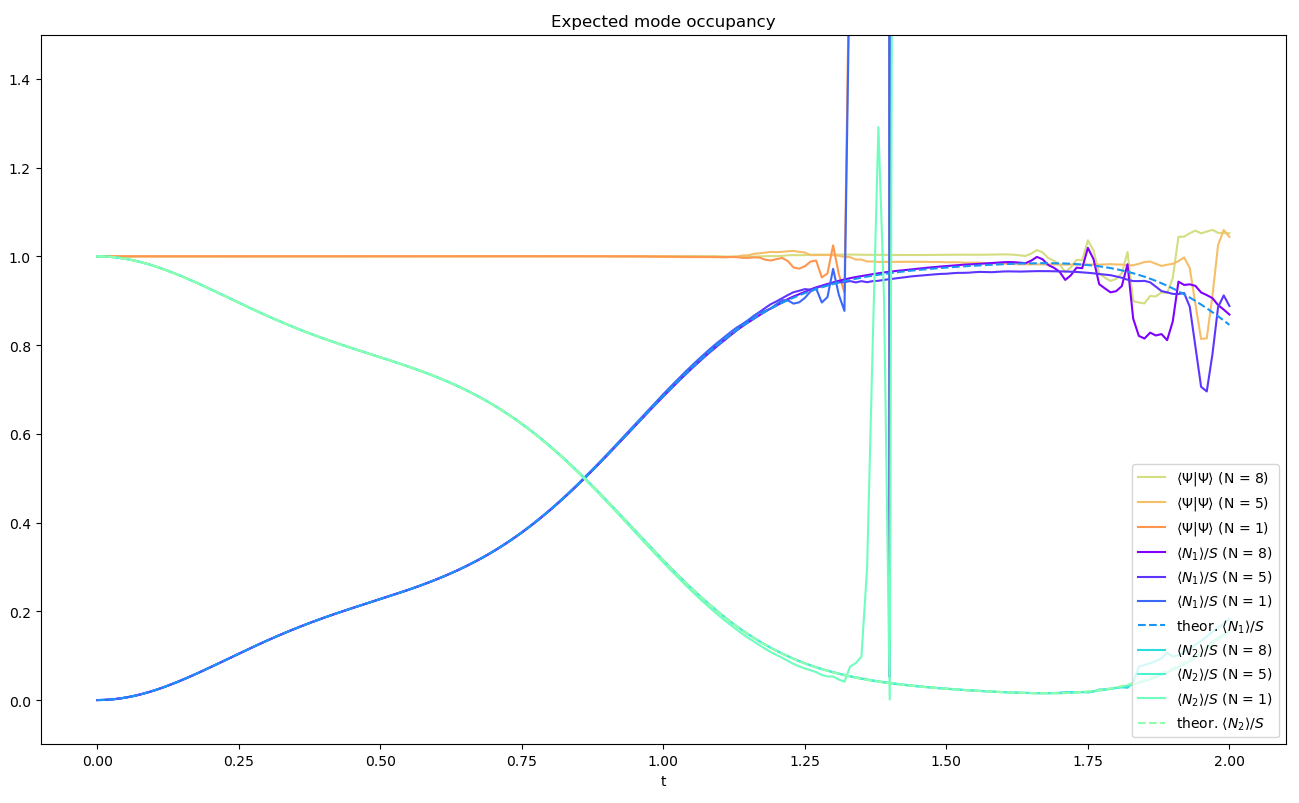
\includegraphics[width=0.85\textwidth]{images/BH_M=2}
	\caption{\textbf{Bose-Hubbard, $M=2$, variational method}. Simulation done with three basis sets, the biggest one being saturated. All three basis sets converged to the true solution, with the two larger ones becoming unstable and diverging at $t=1.3$.}\label{fig:BH_M=2_variational}
	\end{center}
	\end{figure}
	
	\begin{figure}
	\begin{center}
	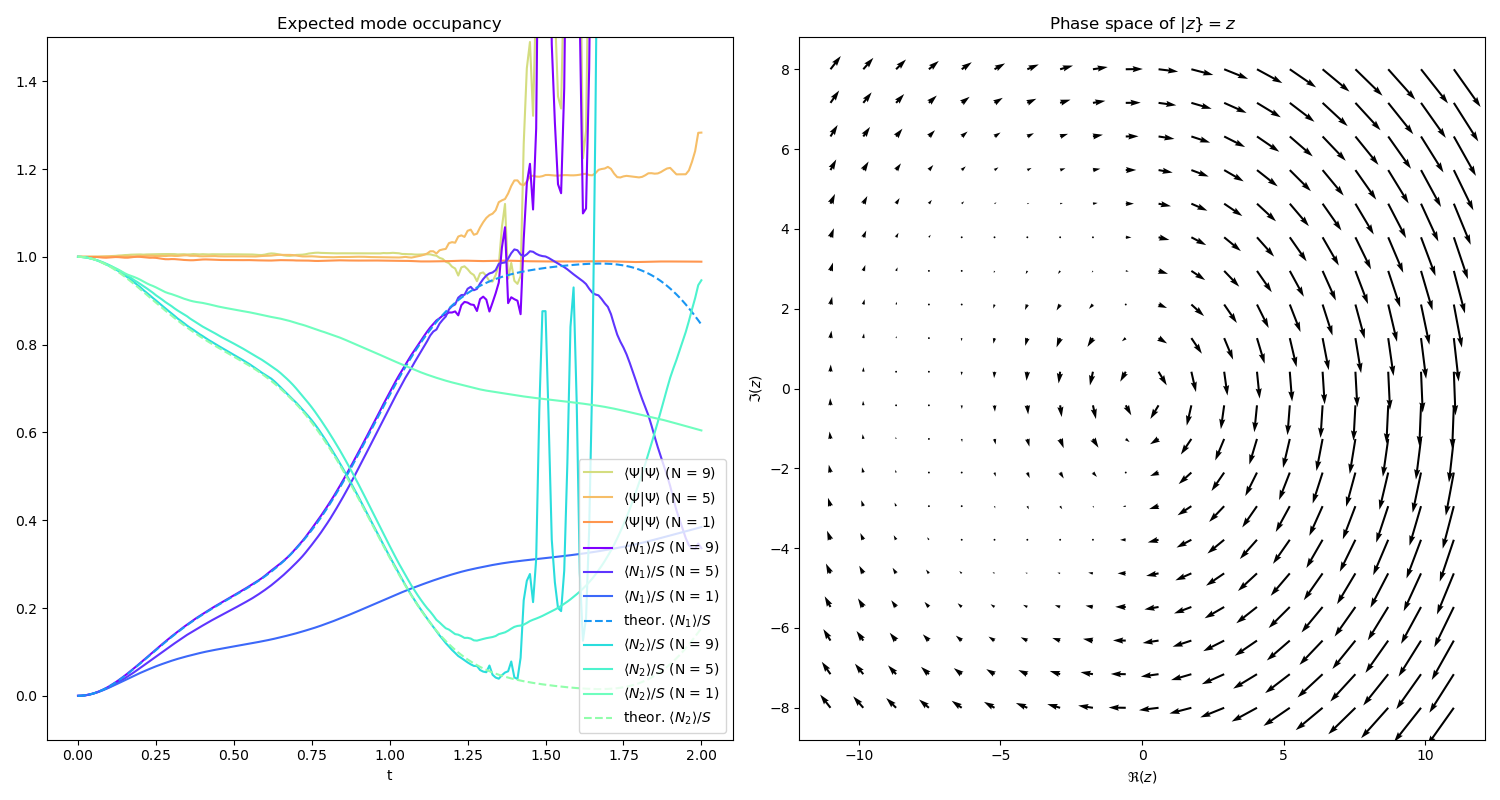
\includegraphics[width=0.85\textwidth]{images/BH_M=2_uncoupled_basis}
	\caption{\textbf{Bose-Hubbard, $M=2$, decoupled basis method}. Here, the two smaller basis sets do not converge, only the $N=9$ set maintaining accuracy. However, this largest basis set becomes unstable and diverges at $t=1.3$.}\label{fig:BH_M=2_uncoupled}
	\end{center}
	\end{figure}
	
	\textbf{Results for $M=3$}
	\begin{itemize}
	\item The results obtained in the first version of the program for the three-mode Bose-Hubbard model using the fully variational method can be seen in Fig. \ref{fig:BH_M=3_variational}
	\item The results for the same system using the decoupled basis method are plotted in Fig. \ref{fig:BH_M=3_uncoupled}.
	\end{itemize}
	
	\begin{figure}
	\begin{center}
	\vspace{-2cm}
	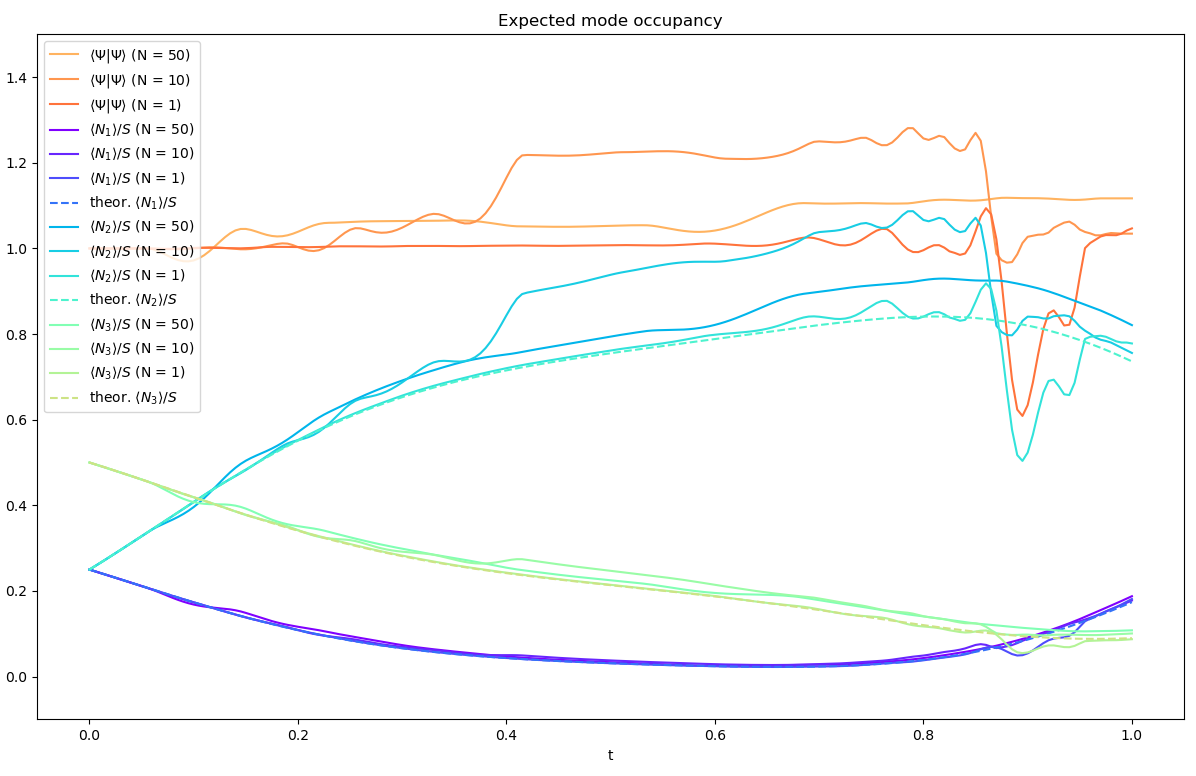
\includegraphics[width=0.85\textwidth]{images/BH_M=3}
	\caption{\textbf{Bose-Hubbard, $M=3$, variational method}. Simulation done with three basis sets, none of them saturated.The smallest basis set converged to the true solution, with the two larger ones becoming unstable and diverging at the beginning of the simulation.}\label{fig:BH_M=3_variational}
	\end{center}
	\end{figure}
	
	\begin{figure}
	\begin{center}
	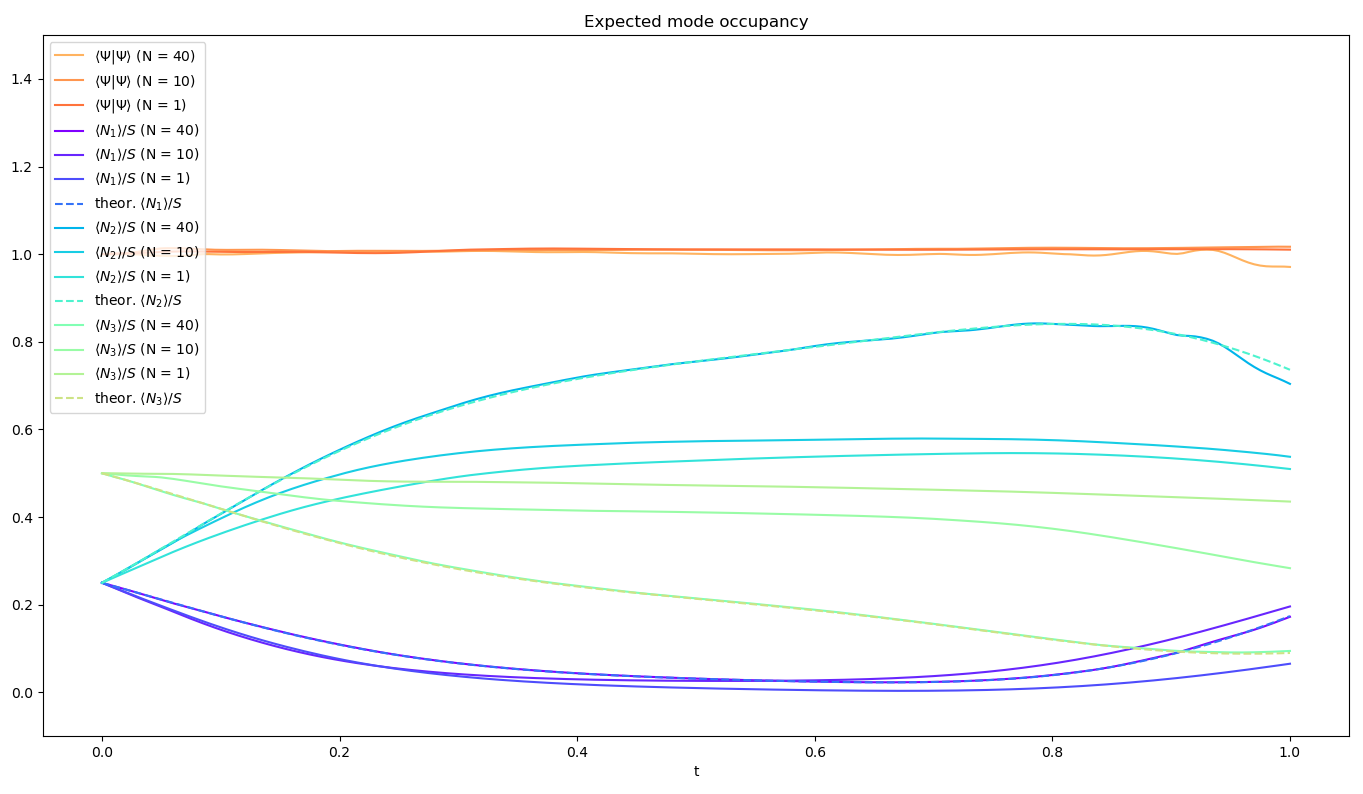
\includegraphics[width=0.85\textwidth]{images/BH_M=3_uncoupled_basis}
	\caption{\textbf{Bose-Hubbard, $M=3$, decoupled basis method}. All three basis sets are stable, but only the largest one ($N=40$) converges.}\label{fig:BH_M=3_uncoupled}
	\end{center}
	\end{figure}
	
	
	\subsubsection{Displaced harmonic trap}
	The Hamiltonian of the displaced harmonic trap is quoted in \cite[Eq. 34]{green}. Using the general form in Eq. \ref{eq:general hamiltonian}, we can express the interaction tensors like so:
	\begin{eqnarray}
	V^{(1)}_{\alpha\beta}&=&\left(\epsilon_{\alpha}+\frac{1}{2}\xi^2\right)\delta_{\alpha,\beta}-\xi Q_{\alpha,\beta}\\
	V^{(2)}_{\alpha\beta\gamma\delta}&=&\lambda_0\delta_{\alpha,\beta,\gamma,\delta}
	\end{eqnarray}
	where $\epsilon_{\alpha}$ is the energy of the mode labelled by $\alpha$ (and is equal to $\frac{1}{2}+\alpha$ in dimensionless units if counting from zero), and $Q_{\alpha,\beta}$ and $\delta_{\alpha,\beta,\gamma,\delta}$ are special tensors defined in \cite[Appendix B]{green}.
	
	Green and Shalashilin analysed the system for two different configurations of physical parameters, one of which I have studied in my results so far: $\xi=2.1,\lambda_0=0.01$.
	
	\textbf{Results for $M=2$}
	\begin{itemize}
	\item The results obtained in the first version of the program for the two-mode displaced harmonic trap model using the fully variational method can be seen in Fig. \ref{fig:DHT_M=2_variational}
	\item The results for the same system using the decoupled basis method are plotted in Fig. \ref{fig:DHT_M=2_uncoupled}.
	\end{itemize}
	
	\begin{figure}
	\begin{center}
	\vspace{-2cm}
	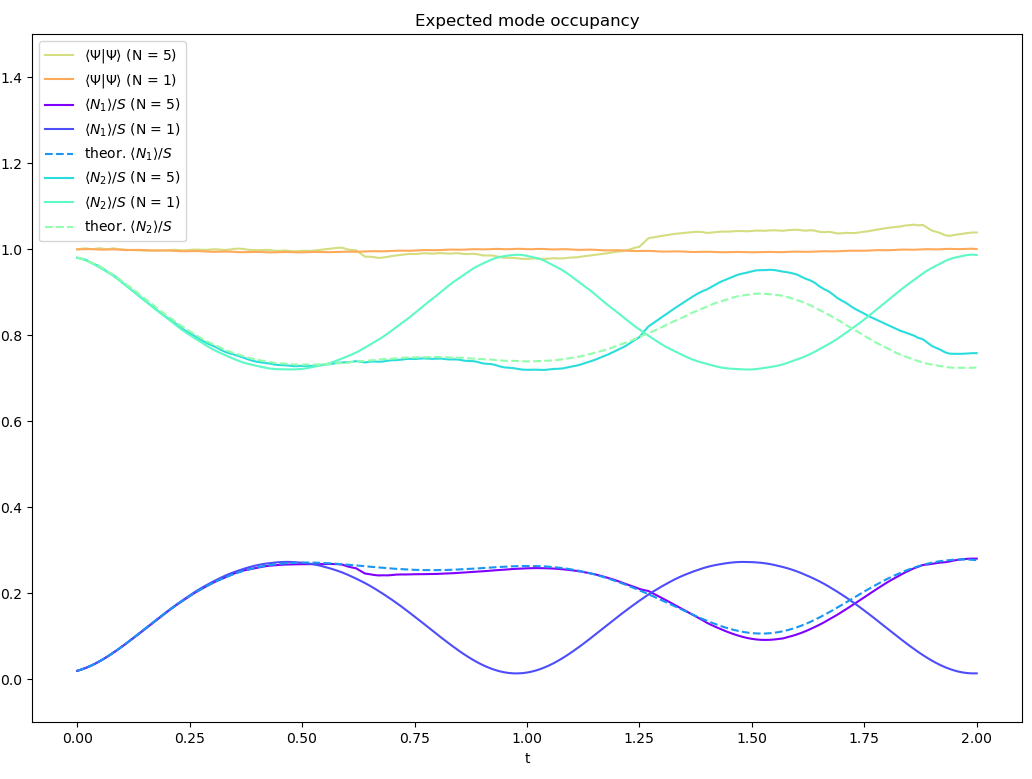
\includegraphics[width=0.82\textwidth]{images/DHT_M=2}
	\caption{\textbf{Displaced harmonic trap, $M=2$, variational method}. Here we only have two basis sets due to quick saturation. Only the larger basis ($N=5$) converges, although not perfectly, due to numerical instability.}\label{fig:DHT_M=2_variational}
	\end{center}
	\end{figure}
	
	\begin{figure}
	\begin{center}
	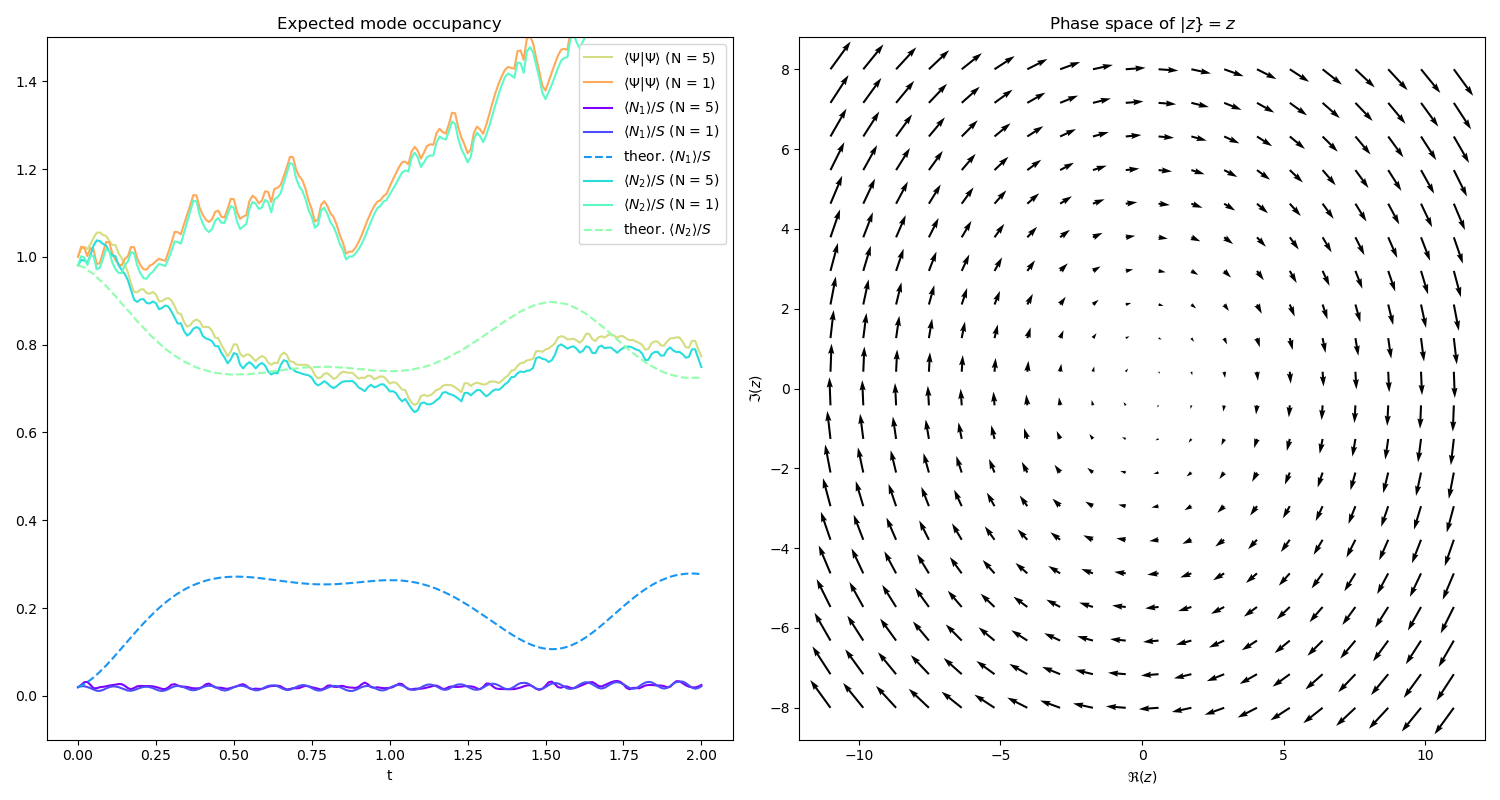
\includegraphics[width=0.82\textwidth]{images/DHT_M=2_uncoupled_basis}
	\caption{\textbf{Displaced harmonic trap, $M=2$, decoupled basis method}. No basis set converges or is numerically stable.}\label{fig:DHT_M=2_uncoupled}
	\end{center}
	\end{figure}
	
	\textbf{Results for $M=3$}
	\begin{itemize}
	\item The results obtained in the first version of the program for the three-mode displaced harmonic trap model using the fully variational method can be seen in Fig. \ref{fig:DHT_M=3_variational}
	\item The results for the same system using the decoupled basis method have not been collected due to issues with numerical stability.
	\end{itemize}
	
	\begin{figure}
	\begin{center}
	\vspace{-2cm}
	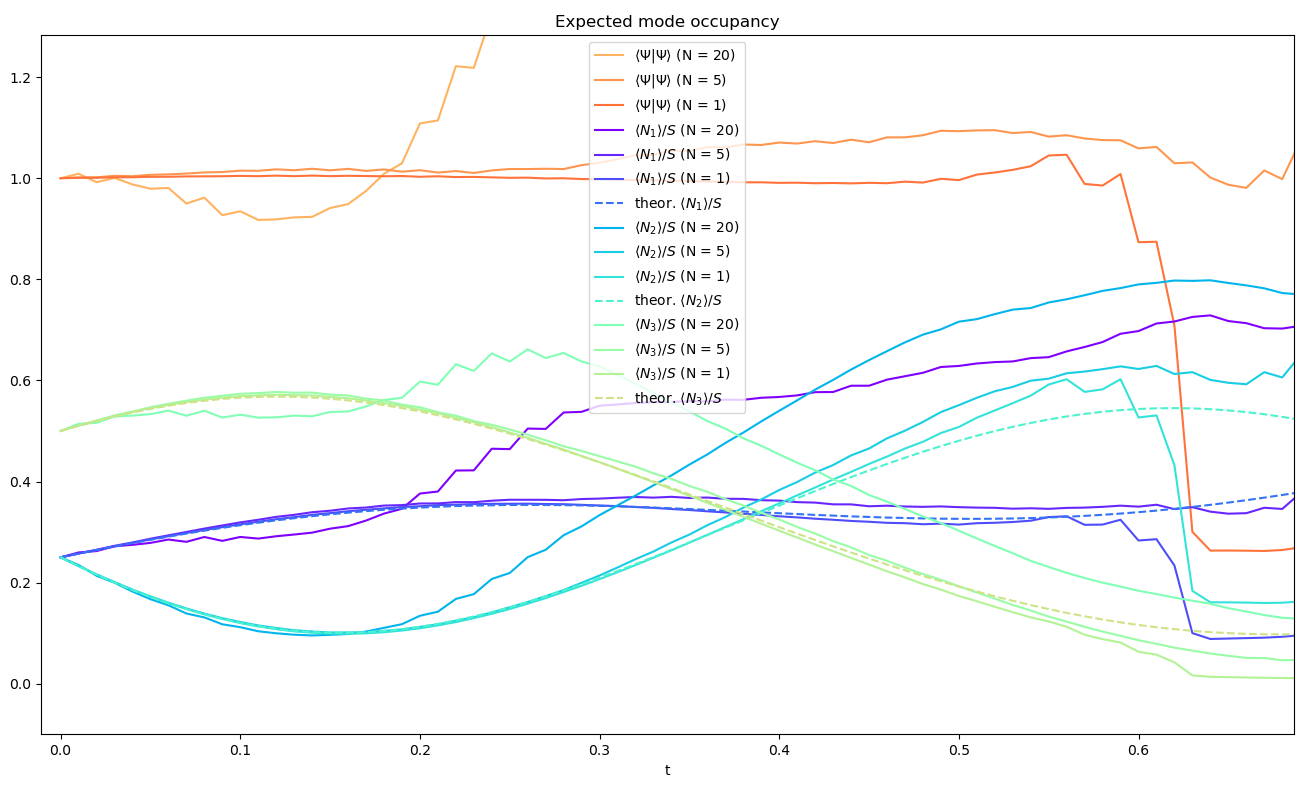
\includegraphics[width=0.85\textwidth]{images/DHT_M=3}
	\caption{\textbf{Displaced harmonic trap, $M=3$, variational method}. The timescale of this simulation is smaller due to numerical instability. The largest basis set ($N=20$) diverges almost immediately. The two smaller basis sets are relatively accurate until they become numerically unstable.}\label{fig:DHT_M=3_variational}
	\end{center}
	\end{figure}
	
	\subsubsection{Discussion of results}
	Both methods are capable of some level of accuracy and stability, with the variational method being very accurate even for small basis sets, but struggling to remain stable, and the decoupled basis method being typically more stable, but less likely to converge to the true result.
	
	It is important to note that all the presented results were collected with benchmark simulation times in the order of minutes on a single-core python routine, and therefore, even without improving the program efficiency, this program can be ran with decreased error tolerance to collect data for comparable mode and particle numbers.
	
	\subsubsection{General remarks}
	For the $M=2$ case, sampling a well-conditioned basis is difficult, as the neighbourhood of the initial wavefunction quickly becomes saturated. This issue becomes easier to deal with for higher values of $S$ and $M$, however, a larger basis is also needed to converge. On the scales I have studied so far, there was no issue with convergence, as even a relatively small basis converged in every scenario. The real issue so far is numerical stability.
	
	The main method to deal with instabilities in the numerical integration process is by decreasing the error tolerance in the Dormand-Prince method, which results in smaller step sizes, i.e. larger number of steps for the simulation to reach the same simulation time. Another method is to study and fine-tune the non-physical simulation parameters, especially the ones related to sampling (i.e. sampling weight function width, maximum conditioning limit, basis size...). A comprehensive study of how to optimalise these parameters, both from a theoretical and a heuristic standpoint, will be conducted to maximise the scope limit of the program.
	
	
	\subsection{Next steps in research}
	The preliminary results are promising, especially as successful demonstrations of the semi-classical approach, since even small basis sets are potentially convergent to the true solution for the complex Hamiltonians we study. However, in order to employ this approach to a larger scale, the challenges of numerical instability and accuracy need to be overcome.
	
	As discussed above, more intelligent sampling and higher computational investment can aid numerical stability, which sets the next goalpost for the research project. Alongside the methods mentioned, there are multiple other methods of aiding the algorithm efficiency, such as
	\begin{itemize}
		\item Dynamic re-sampling of the basis in the case of too high/too low saturation, especially for the decoupled basis method.
		\item Using the semi-classical propagator as stated by Viscondi, Grigolo, and de Aguiar in \cite{Aguiar} to select basis vectors with trajectories that do not dissolve in phase-space, becoming useless to the decomposition propagation.
	\end{itemize}
	
	Although we have so far assumed that the wavefunction is initially in a pure coherent state, this will not generally be the case, especially since this assumption trivialises the problem. Therefore, all of the aforementioned sampling and propagation methods will be chosen in a way which permits an arbitrary initial wavefunction, and will be tested on this regard.
	
	The short-term goal of the project is to fix the issues with numerical stability and convergence, and successfully apply the method of unnormalised $SU(M)$ coherent states to the large-scale version of the systems studied by Qiao and Grossmann, and Green and Shalashilin, respectively. The main focus is to reach the mode number studied by the latter authors for the displaced harmonic trap Hamiltonian.
	
	The long-term goal of the project is to find an analogous approach for fermionic dynamics, which do posses a different dynamical group, the preliminary research on which points out many issues, such as computationally expensive calculation of the overlap matrix.
	
	\subsection{Training plan}
	
	I have participated in several opportunities to connect and communicate with my fellow researchers, such as:
	\begin{itemize}		
		\item attending a COSMOS research group conference, where my supervisor Professor Shalashilin introduced semi-classical, coherent state based methods and their utility in the treatment of quantum-chemical and quantum-molecular dynamics,
		\item communicating with Professor Grossmann, the co-author of one of the papers my research is based in, discussing the similarities and differences in our approaches, and revising the scope and method of my research of coherent state based methods in quantum dynamics,
		\item correspondence with Professor de Aguiar about some of the mathematical nuance in the different treatments of $SU(M)$ coherent states and their effect on the subsequent calculations using the coherent states formalism.
	\end{itemize}
	
	I have also attended several lectures on molecular dynamics and computational chemistry as taught by Professor Shalashilin, as well as the APTC seminar, to get a broader picture of current research in quantum chemistry done by my colleagues.
	
	
	\begin{thebibliography}{10}

	\bibitem{curse_of_dimensionality}
	Shalashilin, D. V. (2011), Multiconfigurational Ehrenfest approach to quantum coherent dynamics in large molecular systems. \textit{Faraday Discussions}, \textbf{153}, pp. 105--116
	
	\bibitem{harmonic_classical_states}
	Schrodinger, E. (1926), Der stetige übergang von der Mikro-zur Makromechanik. \textit{Naturwiss}. 14, pp. 664-666. Translated into English in Schrodinger, E. (1928), \textit{Collected Papers in Wave Mechanics}. 1st edn. London: Blackie \& Son, pp. 41--44
	
	\bibitem{field_coherent_states}
	Glauber, R. J. (1963), Coherent and Incoherent States of the Radiation Field. \textit{Phys. Rev.}, \textbf{131}, 6, pp. 2766--2788
	
	\bibitem{no_unity}
	Klauder, J. R., Skagerstam, B. S. (1985), \textit{Coherent States: Applications in Physics and Mathematical Physics}. 1st eng. edn. Singapore: World Scientific.
	
	\bibitem{perelomov_og}
	Perelomov, A. M. (1972), Coherent states for arbitrary Lie group. \textit{Commun. Math. Phys.}, \textbf{26}, pp. 222--236
	
	\bibitem{gilmore_og}
	Gilmore, R. (1972), Geometry of symmetrized states. \textit{Ann. Phys.}, \textbf{74}, 2, pp. 391--463
	
	\bibitem{ZFG}
	Zhang, W. M., Feng, D. H., Gilmore, R. (1990), Coherent states: Theory and some applications. \textit{Rev. Mod. Phys.}, \textbf{62}, pp. 867--927
	
	\bibitem{Aguiar}
	Viscondi, T. F., Grigolo, A., de Aguiar, M. A. M. (2015), Semiclassical Propagator in the Generalized Coherent-State Representation. \href{https://doi.org/10.48550/arXiv.1510.05952}{arXiv:1510.05952 \textbf{[quant-ph]}}
	
	\bibitem{optical_lattices}
	Block, I., Dalibard, J., Zwerger, W. (2008), Many-body physics with ultracold gases. \textit{Rev. Mod. Phys.}, \textbf{80}, pp. 885--964
	
	\bibitem{grossmann}
	Qiao, Y., Grossmann, F. (2021), Exact variational dynamics of the multimode Bose-Hubbard model based on $SU(M)$ coherent states. \textit{Phys. Rev. A}, \textbf{103}, 042209
	
	\bibitem{green}
	Green, J. A., Shalashilin, D. V. (2019), Simulation of the quantum dynamics of indistinguishable bosons with the method of coupled coherent states. \textit{Phys. Rev. A}, \textbf{100}, 013607
	
	\bibitem{gellmann}
	Bertlmann, R. A., Krammer, P. (2008), Bloch vectors for qudits. \href{ 	
https://doi.org/10.48550/arXiv.0806.1174}{arXiv:0806.1174 \textbf{[quant-ph]}}

	\bibitem{buonsante}
	Buonsante, P., Penna, V.(2008), Some remarks on the coherent-state variational approach to nonlinear boson models. \textit{J. Phys. A: Math. Theor.}, \textbf{41}, 175301
	
	\bibitem{sampling_algorithm}
	Grigolo, A., Viscondi, T. F., de Aguiar, M. A. M. (2016), Multiconfigurational quantum propagation with trajectory-guided generalized coherent states. \textit{J. Chem. Phys.}, \textbf{144}, 094106

	\end{thebibliography}
	\bibliographystyle{unsrt}
	
	
	
	

	
	
\end{document}